% ============================================================================
% Phase 2 Research Report - FedZT-Edge
% Extended Literature Review, Refined Research Gap, and Research Methodology
% ----------------------------------------------------------------------------
% HOW TO COMPILE
%   * Overleaf: upload this single file, set compiler to pdfLaTeX, compile x2.
%   * Local:    pdflatex main.tex  (run twice for TOC + cross-references)
%   * Self-contained: no external images or .bib files required.
% EDIT BEFORE SUBMISSION: replace [Student Name] and [Supervisor Name] on the
%   title page, and confirm the three core-paper entries marked "% TODO" in
%   the references against your Phase 1 report.
% ============================================================================
\documentclass[11pt,a4paper]{article}

% ---------- Core packages (hyperref loads last among content packages) ------
\usepackage[T1]{fontenc}
\usepackage[utf8]{inputenc}
\usepackage{lmodern}
\usepackage{geometry}
\geometry{a4paper, top=2.5cm, bottom=2.5cm, left=2.5cm, right=2.5cm}
\usepackage{graphicx}
\usepackage{xcolor}
\usepackage{amsmath}
\usepackage{booktabs}
\usepackage{tabularx}
\usepackage{longtable}
\usepackage{array}
\usepackage{enumitem}
\usepackage{pdflscape}
\usepackage{needspace}
\usepackage[numbers,sort&compress]{natbib}
\usepackage{tikz}
\usetikzlibrary{arrows.meta,positioning,calc}
\usepackage{fancyhdr}
\usepackage[colorlinks=true,linkcolor=blue!55!black,citecolor=blue!55!black,
            urlcolor=blue!55!black,bookmarks=true,bookmarksnumbered=true,
            unicode=true]{hyperref}
\usepackage{tcolorbox}

% ---------- Typography and layout hygiene -----------------------------------
\widowpenalty=10000
\clubpenalty=10000
\emergencystretch=1.5em
\setlength{\parskip}{4pt}
\setlength{\parindent}{0pt}
\renewcommand{\arraystretch}{1.2}
\setlength{\headheight}{14pt}

\pagestyle{fancy}
\fancyhf{}
\fancyhead[L]{\small\itshape Phase 2 Research Report --- FedZT-Edge}
\fancyhead[R]{\small\thepage}
\renewcommand{\headrulewidth}{0.4pt}

% Ragged-right narrow table column (avoids underfull justification gaps)
\newcolumntype{L}[1]{>{\raggedright\arraybackslash}p{#1}}

% PDF metadata (must be in the preamble for xdvipdfmx to write it)
\hypersetup{
  pdftitle={FedZT-Edge Phase 2 Research Report: Extended Literature Review,
            Refined Research Gap, and Research Methodology},
  pdfauthor={[Student Name]},
  pdfsubject={Federated Zero-Trust WebAssembly Intrusion Detection for Edge
              Networks},
  pdfkeywords={federated learning, intrusion detection, zero trust,
               WebAssembly, DRL, non-IID, edge computing}
}

% Accent colours (low-saturation, print friendly)
\definecolor{accent}{HTML}{1F4E79}
\definecolor{layerblue}{HTML}{EFF6FF}
\definecolor{layergreen}{HTML}{F0FDF4}
\definecolor{layeramber}{HTML}{FFFBEB}
\definecolor{layerviolet}{HTML}{F5F3FF}
\definecolor{layerrose}{HTML}{FFF1F2}

% Highlight box for the research gap statement
\newtcolorbox{gapbox}[1][]{colback=accent!4,colframe=accent,boxrule=0.9pt,
  arc=2pt,left=8pt,right=8pt,top=8pt,bottom=8pt,#1}

% Section helper: never start a major section in the bottom quarter of a page
% (starred \Needspace* is used because unstarred \needspace mis-measures
% after rotated landscape pages and forces spurious page breaks)
\newcommand{\bigsection}[1]{\Needspace*{0.22\textheight}\section{#1}}

% ============================================================================
\begin{document}

% ----------------------------------------------------------------------------
% TITLE PAGE (portable LaTeX-native layout; no \maketitle)
% ----------------------------------------------------------------------------
\thispagestyle{empty}
\begin{center}
\vspace*{2.2cm}
{\color{accent}\rule{\textwidth}{1.2pt}}\\[10pt]
{\LARGE\bfseries FedZT-Edge: A Federated, Zero-Trust,\\[4pt]
WebAssembly-Based Intrusion Detection Framework\\[4pt]
for Resource-Constrained Edge Networks\par}
\vspace{10pt}
{\Large Phase 2 Research Report\par}
\vspace{6pt}
{\large Extended Literature Review, Refined Research Gap,\\
and Research Methodology\par}
\vspace{10pt}
{\color{accent}\rule{\textwidth}{1.2pt}}
\vspace{1.6cm}

{\large\bfseries [Student Name]\par}
\vspace{4pt}
{\normalsize Department of Computer Science\\
FAST National University of Computer and Emerging Sciences (FAST-NUCES)\par}
\vspace{4pt}
{\normalsize Supervisor: [Supervisor Name]\par}
\vspace{1.5cm}

{\normalsize Deliverables covered in this report:\par}
\begin{itemize}[leftmargin=2.2em,itemsep=2pt]
  \item[\textbf{D1}] Extended literature review with ten new studies (2025--2026)
  \item[\textbf{D2}] Refined and justified research gap statement
  \item[\textbf{D3}] Step-by-step research methodology (twelve steps)
  \item[\textbf{D4}] Methodology and architecture diagrams
\end{itemize}
\vfill
{\normalsize October 2025\par}
\vspace{0.8cm}
\end{center}
\newpage

% ----------------------------------------------------------------------------
\tableofcontents
\newpage

% ============================================================================
\bigsection{Introduction and Phase 2 Objectives}\label{sec:intro}
% ============================================================================

Phase~1 of this project established the foundation of the proposed work by
analysing three core studies in depth: FLEX-IDS, a federated and explainable
intrusion detection system (IDS) for Edge-of-Things environments under
adversarial conditions~\cite{flexids}; the DQN-based deep reinforcement
learning (DRL) Zero-Trust security framework of Mahida et
al.~\cite{mahida2026}; and the Rust/WebAssembly (Wasm) edge-IDS benchmarking
framework of Weber et al.~\cite{weber2026}. That analysis exposed three
persistent weaknesses in the current literature. First, federated IDS
pipelines are rarely evaluated under adversarial client behaviour such as
label-flipping poisoning. Second, experiments are almost always conducted
under independent and identically distributed (IID) data assumptions that do
not reflect heterogeneous edge deployments. Third, no study unifies
federated learning (FL), DRL-driven Zero-Trust mitigation, and
Wasm-level lightweight execution in a single architecture that is evaluated
jointly for security and resource cost.

Phase~2 converts those observations into a concrete, defensible research
plan. This report delivers four artefacts. Section~\ref{sec:litreview}
presents deliverable D1, an extended literature review that adds ten new
studies published between 2025 and 2026, together with a verified comparison
table. Section~\ref{sec:gap} presents deliverable D2, the refined research
gap statement and its evidence-based justification.
Section~\ref{sec:method} presents deliverable D3, a twelve-step research
methodology spanning data preparation, the five-layer FedZT-Edge
architecture, baselines, experimental design, metrics, statistics,
ablations, and outputs. Section~\ref{sec:diagram} presents deliverable D4,
the methodology and architecture diagrams that visualise the plan.

One practical constraint shaped the sourcing strategy of this phase: the
FAST-NUCES institutional email does not provide IEEE Xplore or comparable
subscription access beyond open-access venues. All primary sources
therefore needed to be either freely downloadable or clearly marked as
citation-only. Seven of the ten new studies were obtained and verified from
full open-access text, while three (Refs.~\cite{rezaei2025,bensaid2025,nandanwar2025})
remain paywalled and are integrated at abstract and metadata level, with
their table entries explicitly flagged. This transparency rule keeps every
claim in the review traceable to material that was actually read, which is
essential for the credibility of the gap argument developed in
Section~\ref{sec:gap}.

% ============================================================================
\bigsection{Extended Literature Review (Deliverable D1)}\label{sec:litreview}
% ============================================================================

\subsection{Selection Method and Evidence Sources}\label{sec:selection}

The ten new studies were selected through a two-stage process. In the first
stage, forward and backward citation snowballing was applied to the three
Phase~1 core papers~\cite{flexids,mahida2026,weber2026} to capture work that
cites or is cited by the direct ancestors of the proposed research. In the
second stage, targeted queries were issued against open-access repositories
(Nature Scientific Reports, MDPI, Springer Open, IEEE Access, and arXiv)
using keyword combinations such as \emph{federated intrusion detection},
\emph{label flipping}, \emph{non-IID}, \emph{WebAssembly runtime}, and
\emph{edge IDS}. Studies published between 2025 and 2026 were preferred so
that the review reflects the current state of the field, and each candidate
was retained only if it either (i) provided a full open-access text that
could be downloaded and extracted, or (ii) was indispensable for a specific
gap dimension, in which case it was integrated at abstract level and
flagged.

This procedure produced ten studies: seven verified from full text
(Refs.~\cite{albogami2025,karunamurthy2025,berguiga2025,zhang2025,djemaa2026,hozouri2025,diana2025})
and three integrated from citations and abstracts
(Refs.~\cite{rezaei2025,bensaid2025,nandanwar2025}). Two substitution
decisions are worth recording. The originally shortlisted Mihaylova
conference paper on adversarial attacks against network IDS proved to be
available only under a paywalled IEEE proceedings licence, so it was
replaced by the substantially broader and fully open-access heterogeneity
survey of Djemaa et al.~\cite{djemaa2026}, which covers the same attack
surface (poisoning and evasion) with an explicit non-IID lens. Likewise,
the blockchain-assisted IDS of Nandanwar et al.~\cite{nandanwar2025} could
not be obtained freely and is retained as a citation-only supporting study,
since the collaborative-IDS angle it represents is already covered in depth
by the open survey of Diana et al.~\cite{diana2025}. All cells of the
comparison table in Section~\ref{sec:comptable} that rest on full-text
extraction were verified directly against the downloaded PDFs, which
corrected several preliminary entries that had been inferred from citing
context in the earlier draft of this review.

\subsection{Federated IDS Architectures (Albogami, Karunamurthy, Bensaid)}
\label{sec:flids}

Albogami~\cite{albogami2025} proposes IDFLM-ES, an intelligent deep
federated learning model for IoT-enabled edge computing. The detector is a
federated hybrid deep belief network (FHDBN) trained on time-series data
produced by IoT edge devices, preceded by min--max normalisation and
Golden Jackal Optimization (GJO) for feature selection, and followed by
Dung Beetle Optimization (DBO) for hyperparameter tuning. Experiments on a
curated subset of Edge-IIoTset containing 15{,}000 samples across 15
balanced classes report an average accuracy of 98.24\%, an F1-score of
86.77\%, and a computational time of 10.55~s, outperforming CNN, RNN, KNN,
ANN, Naive Bayes, and SVM comparators. The study is a useful architectural
reference for FedZT-Edge because it demonstrates metaheuristic feature
selection and hyperparameter tuning inside an FL loop. However, its
evaluation is entirely IID, it reports no adversarial scenarios, and it
offers no per-device energy, latency, or memory measurements, which limits
its transferability to genuinely constrained hardware.

Karunamurthy et al.~\cite{karunamurthy2025} present an FL-based IDS in
which each IoT client trains a local CNN on an optimally selected feature
subset produced by the Chimp Optimization Algorithm, after which a central
server aggregates client parameters into a global model. Evaluation on a
benchmark MQTT-oriented dataset yields a maximum detection accuracy of
95.59\% with an average precision of 0.9479, exceeding decision tree,
random forest, neural network, gradient boosting, and Naive Bayes
baselines. The paper is valuable to this project in two ways: it confirms
the feasibility of CNN-level local training on reduced feature sets, and
its related-work experiments on Edge-IIoT (92.49\% accuracy) provide a
useful cross-dataset anchor. Its limitations mirror those of
Ref.~\cite{albogami2025}: the partitioning is IID, no attacks are launched
against the FL process itself, and no edge hardware benchmark is reported.

Bensaid et al.~\cite{bensaid2025} (integrated at abstract level) address
fog-assisted smart-home security with 2FIDS, a federated learning-based
intrusion detection approach in which LSTM-based local learning is
combined with secure fog-level aggregation over TLS-protected channels.
The fog hierarchy is directly relevant to FedZT-Edge because it positions
detection between constrained endpoints and the cloud, and it motivates the
policy-enforcement-point (PEP) placement adopted in
Section~\ref{sec:arch}. Because the full text remains behind a Springer
paywall, its dataset composition, partitioning strategy, and robustness
results could not be independently verified, and its table row in
Section~\ref{sec:comptable} is therefore marked as abstract-level.

\subsection{Adversarial Robustness and Heterogeneity (Rezaei, Djemaa)}
\label{sec:robust}

Rezaei et al.~\cite{rezaei2025} (integrated at abstract level) study a
federated RNN intrusion detector for IoT environments that continues to
operate under adversarial attack, with a defence lineage that filters
suspicious client updates using Gaussian mixture model (GMM) scoring and
K-means clustering before aggregation. This line of work is the closest
published ancestor of the robustness layer planned for FedZT-Edge, because
it treats the FL aggregation server itself as an attack surface and
demonstrates that poisoning defence can be decoupled from the detector
architecture. The paywalled status of the Journal of Network and Systems
Management prevents full verification of its datasets, attack
parameterisation, and quantitative gains, so its contribution is used
qualitatively to justify the design choice in Step~5 of the methodology
rather than as a quantitative baseline.

Djemaa, Djenouri, and Legg~\cite{djemaa2026} provide the most directly
relevant robustness evidence in the new corpus. Their survey follows a
PRISMA-style protocol that screened 1{,}850 records down to a final
evidence base of 130, and it makes a central argument that aligns exactly
with the motivation of this project: poisoning mitigation cannot be
evaluated only by attack type, defence family, or clean accuracy, but must
also be assessed against the channel through which a
heterogeneity-shaped attack is expressed. The survey formalises six
heterogeneity dimensions (statistical, model and knowledge distillation,
task and objective, device and resource, communication, and participation)
and shows how each one changes attack feasibility, stealth, persistence,
and detectability, while benign clients with unusual but legitimate
updates are at risk of being filtered by anomaly-based defences. It
further proposes operational comparison criteria --- attack--defence
alignment, evidence validity, server visibility, privacy compatibility,
scalability, deployment feasibility, and benign-client preservation ---
that FedZT-Edge adopts directly in its evaluation plan
(Section~\ref{sec:stats}). Crucially for the gap argument, the survey
concludes that no existing work jointly evaluates poisoning defences,
intrusion detection workloads, and edge resource constraints, and it
explicitly lists IDS clients as a domain where heterogeneity is strongest.

\subsection{Lightweight Edge Execution: WebAssembly and Device-Level IDS
(Zhang, Berguiga)}\label{sec:wasm}

Zhang et al.~\cite{zhang2025} deliver the first comprehensive survey of
Wasm runtimes, covering 98 studies collected between 2017 and early 2024
(published version in ACM TOSEM; the arXiv v2 preprint was used for this
review because it is freely accessible). The survey organises the field
into internal research (runtime design, testing, and analysis: 52 design
studies, 33 testing studies, and 13 analysis studies) and external
application research, of which edge computing (11 studies), IoT (7
studies), and trusted execution environments (8 studies) are the domains
closest to this project. Its empirical highlights quantify both the promise
and the cost of Wasm at the edge: sandboxed Kubernetes controllers built on
Wasmtime reduce memory usage by 64\%; the Wasmachine runtime executes
Wasm binaries 11\% faster than native Linux execution on IoT and fog
devices thanks to ahead-of-time compilation and zero-cost system calls;
Wasm execution saves 20--30\% energy relative to equivalent JavaScript;
and micro-benchmarks still show a 5--10$\times$ performance loss versus
native execution for general workloads. The survey also profiles the five
dominant standalone runtimes (Wasmtime, Wasmer, WAMR, WasmEdge, wasm3) by
interpreter, JIT, and AoT capability, which informs the runtime selection
and fuel-metering configuration in Section~\ref{sec:arch}. Its decisive
limitation for our purposes is scope: none of the 98 studies benchmarks an
intrusion detection workload under FL-produced models, so the Wasm
execution cost of IDS inference remains unmeasured in the literature.

Berguiga, Harchay, and Massaoudi~\cite{berguiga2025} demonstrate the
device-level counterpart of this execution story with HIDS-IoMT, a hybrid
deep learning IDS that combines a CNN for feature extraction with an LSTM
for sequence prediction and is deployed on a Raspberry Pi inside a fog
architecture for Internet of Medical Things networks. Using the IoTID20
and Edge-IIoTset datasets against DDoS, SQL injection, vulnerability
scanner, port scanning, and Mirai attack families, the model reaches
99.92\% accuracy, 99.91\% precision, 99.99\% recall, and an F1-score of
99.95\%. The study is included in this review primarily as evidence that
(i) realistic deep IDS models can run on single-board computers, and (ii)
fog-level placement measurably reduces latency for latency-sensitive
applications. Two contrasts with FedZT-Edge are instructive. First,
HIDS-IoMT is trained centrally and merely deployed at the edge; it has no
federated dimension at all. Second, it reports detection quality but no
fuel, memory, or energy instrumentation of the kind that a Wasm-based
execution layer makes possible, so its edge claims cannot be converted
into comparable resource metrics.

\subsection{Surveys, Datasets, and Supporting Technologies (Hozouri,
Diana, Nandanwar)}\label{sec:surveys}

Hozouri, Mirzaei, and Effatparvar~\cite{hozouri2025} survey IDS research
across machine learning and deep learning methods, organising the field by
detection paradigm, architecture, and evaluation dataset, with particular
attention to CIC-IDS2017, KDDCup99, and UNSW-NB15. The survey includes a
dedicated treatment of adversarial machine learning --- evasion and
poisoning attacks, and the trade-off between adversarial training and
input sanitisation as defences --- which supports the threat taxonomy
adopted in Step~5 of the methodology. Its stated conclusion, that scalable
and adaptable IDS solutions for evolving threats remain an open research
need, corroborates the gap refined in Section~\ref{sec:gap} from the
survey side. For this project the paper also serves as the dataset
justification reference: it documents why UNSW-NB15 remains a standard
benchmark despite known staleness issues, which is one of the two primary
datasets selected for FedZT-Edge.

Diana, Dini, and Paolini~\cite{diana2025} offer a broad-spectrum IDS
review spanning signature-, anomaly-, and specification-based detection;
host-, network-, and hybrid architectures; and deployments in cloud,
virtualised, IoT, and industrial control system environments. Two of its
threads matter here. First, its treatment of collaborative and
blockchain-assisted IDS --- including federated deep learning systems such
as DeepFed evaluated on Edge-IIoTset and the Passban edge IDS --- shows
that decentralised trust scaffolding around detection is an active
research direction, which the citation-only study of Nandanwar et
al.~\cite{nandanwar2025} extends with a hybrid blockchain framework for
IoT intrusion detection. Second, its challenges section identifies
scalability, false-positive reduction, adversarial resilience, and the
shift toward autonomous, proactive IDS as the defining open problems,
which is precisely the niche that the DRL-driven mitigation layer of
FedZT-Edge is designed to occupy. Neither survey, however, connects these
threads to each other or to Wasm-level execution economics, which keeps
the unified gap open.

\subsection{Comparative Summary of the Ten New Studies}\label{sec:comptable}

Table~\ref{tab:comparison} consolidates the review into a single matrix.
Rows marked with a dagger ($\dagger$) are integrated from citation and
abstract material only, because no legal open-access full text exists at
the time of writing; all other rows were verified against the downloaded
PDFs. The capability columns (non-IID, adversarial robustness, edge or
Wasm deployment) record whether the study actually \emph{evaluates} the
capability, not merely whether it mentions it.

\begin{landscape}
\begingroup
\footnotesize
\setlength{\tabcolsep}{4pt}
\setlength{\LTleft}{\fill}
\setlength{\LTright}{\fill}
% longtable splits across landscape pages (a fixed tabular would silently
% lose rows that do not fit), and hard-coded [n] citations avoid link
% annotations on the rotated page, which xdvipdfmx would place outside the
% portrait MediaBox.
\begin{longtable}{L{2.9cm}L{3.1cm}L{2.4cm}L{2.6cm}L{1.3cm}L{2.1cm}L{2.7cm}L{4.4cm}}
\caption{Verified comparison of the ten new studies added in Phase 2.
$\dagger$ = abstract-level entry (no open-access full text). n/a indicates
dimensions not applicable to survey papers.}
\label{tab:comparison}\\
\toprule
\textbf{Study / venue} & \textbf{Approach and model} & \textbf{Dataset(s)} &
\textbf{FL / aggregation} & \textbf{Non-IID} & \textbf{Adversarial robust.} &
\textbf{Edge / Wasm deployment} & \textbf{Key results and limitations} \\
\midrule
\endfirsthead
\multicolumn{8}{l}{\footnotesize\itshape Table~\ref{tab:comparison} continued from previous page}\\
\toprule
\textbf{Study / venue} & \textbf{Approach and model} & \textbf{Dataset(s)} &
\textbf{FL / aggregation} & \textbf{Non-IID} & \textbf{Adversarial robust.} &
\textbf{Edge / Wasm deployment} & \textbf{Key results and limitations} \\
\midrule
\endhead
\midrule
\multicolumn{8}{r}{\footnotesize\itshape continued on next page}\\
\endfoot
\bottomrule
\endlastfoot
Rezaei et al.\ 2025 [4], J.\ Netw.\ Syst.\ Manage.\ $\dagger$ &
Fed-RNN IDS under label-flipping attack; GMM + K-means filtering of
suspicious client updates & not extractable (paywalled) & FedAvg-based FL
with update filtering & not stated & yes --- label flipping (defense
proposed) & no & Robustness-oriented design; quantitative gains not
independently verified. \\
\addlinespace[2pt]
Bensaid et al.\ 2025 [5], Cluster Comput.\ $\dagger$ &
2FIDS: fog-assisted FL-IDS; LSTM local models; secure TLS aggregation &
smart-home IoT traffic & hierarchical fog FL & not stated & not stated &
fog nodes (no Wasm) & Fog-level aggregation for smart homes; dataset and
robustness details unverified. \\
\addlinespace[2pt]
Albogami 2025 [6], Sci.\ Rep.\ 15:4041 &
IDFLM-ES: federated hybrid deep belief network; GJO feature selection; DBO
hyperparameter tuning & Edge-IIoTset subset (15{,}000 samples, 15 classes) &
FedAvg-style averaging of local HDBNs & no (IID) & no & edge devices
(simulation; no hardware metrics) & Acc.\ 98.24\%, F1 86.77\%, CT 10.55~s;
IID-only, no adversarial tests, no energy model. \\
\addlinespace[2pt]
Karunamurthy et al.\ 2025 [7], Sci.\ Rep.\ 15:8696 &
FLIDS: local CNN + Chimp Optimization feature selection; central
aggregation & MQTT benchmark (ToN-IoT oriented) & FedAvg-style CNN weight
aggregation & no & no & IoT devices (simulation) & Acc.\ 95.59\%, precision
94.79\%; beats DT/RF/NB/GB; IID-only, no FL attacks, no hardware
profiling. \\
\addlinespace[2pt]
Nandanwar et al.\ 2025 [8], Cluster Comput.\ $\dagger$ &
Hybrid blockchain-assisted IDS framework for IoT & IoT traffic &
blockchain-assisted decentralised detection & not stated & immutability /
audit focus & not stated & Integrity and auditability layer for
collaborative IDS; details unverified. \\
\addlinespace[2pt]
Berguiga et al.\ 2025 [9], IEEE Access &
HIDS-IoMT: CNN feature extraction + LSTM sequence prediction & IoTID20,
Edge-IIoTset & none (centralised) & no & no & Raspberry Pi, fog
architecture (real device) & Acc.\ 99.92\%, F1 99.95\%; not federated; no
fuel, memory, or energy instrumentation. \\
\addlinespace[2pt]
Zhang et al.\ 2025 [10], ACM TOSEM / arXiv &
Survey of 98 Wasm-runtime studies: design (52), testing (33), analysis
(13) & n/a (survey) & n/a & n/a & sandboxing and security analysis &
Wasmtime, Wasmer, WAMR, WasmEdge, wasm3; edge and IoT scenarios & Edge
findings: $-64\%$ memory, $+11\%$ faster than native (Wasmachine), 20--30\%
energy saving vs JS, 5--10$\times$ native gap; no IDS-specific Wasm
benchmark. \\
\addlinespace[2pt]
Djemaa et al.\ 2026 [11], Electronics 15(13):2876 &
Survey and taxonomy: poisoning attacks $\times$ heterogeneity;
attack--defence alignment criteria & n/a (130-record evidence base) & FL
settings throughout & yes --- core focus (six dimensions) & yes ---
label-flipping, backdoor, Byzantine, Sybil & deployment constraints
(edge/IoT) discussed & No IDS-specific joint evaluation; no edge resource
measurement; defines open challenges adopted by this project. \\
\addlinespace[2pt]
Hozouri et al.\ 2025 [12], Discov.\ Artif.\ Intell.\ 5:314 &
Survey: ML/DL IDS taxonomy + adversarial ML section & reviews CIC-IDS2017,
KDDCup99, UNSW-NB15 & FL discussed & discussed & discussed & n/a &
Concludes scalable, adaptable IDS for evolving threats remains open;
supports UNSW-NB15 dataset choice. \\
\addlinespace[2pt]
Diana et al.\ 2025 [13], Computers 14(3):87 &
Broad IDS review: signature / anomaly / specification; cloud, IoT, ICS,
SDN; blockchain collaborative IDS & reviews standard IDS datasets & FL and
blockchain collaborative IDS covered & n/a & adversarial resilience as
challenge & edge IDS (Passban) discussed & Challenges: scalability,
false positives/negatives, zero-day; proactive IDS trend; no unified
stack. \\
\end{longtable}
\endgroup
\end{landscape}

\subsection{Synthesis of the New Evidence}\label{sec:synthesis}

Read together, the ten studies sharpen the picture that motivated Phase~1
rather than closing it. The three federated detection
studies~\cite{albogami2025,karunamurthy2025,bensaid2025} confirm that
modern detectors --- hybrid DBNs, CNNs, and LSTMs --- can be trained under
federated averaging with feature selection, but every one of them
partitions its data in an IID fashion, launches no attack against the FL
process, and measures nothing about the hardware it claims to serve. The
robustness strand~\cite{rezaei2025,djemaa2026} establishes both the
mechanism (statistical filtering of client updates) and the evaluation
vocabulary (attack--defence alignment under heterogeneity), yet couples
neither to a concrete intrusion detection deployment with resource
budgets. The execution strand~\cite{zhang2025,berguiga2025} proves that
sandboxed, instrumented inference on single-board computers is practical
and that Wasm runtimes are mature enough to be chosen between, but the
Wasm literature has never been fused with federated model delivery, and
the device-level IDS literature reports accuracy without fuel, memory, or
energy accounting. Finally, the survey
strand~\cite{hozouri2025,diana2025,nandanwar2025} maps the datasets,
attack taxonomies, and collaborative scaffolding that a credible proposal
must build on. The capability columns of Table~\ref{tab:comparison} make
the resulting void visible at a glance: no row simultaneously ticks the
non-IID, adversarial robustness, and edge/Wasm deployment columns, which
is exactly the intersection that Section~\ref{sec:gap} formalises.

% ============================================================================
\bigsection{Refined Research Gap (Deliverable D2)}\label{sec:gap}
% ============================================================================

The extended review in Section~\ref{sec:litreview} permits a sharper
formulation of the research gap than the preliminary statement produced at
the end of Phase~1. The refined statement, which guides every design
decision in Section~\ref{sec:method}, is:

\begin{gapbox}
\textbf{Refined gap statement.} \emph{No existing 2025--2026 study unifies
federated intrusion detection, DRL-based adaptive Zero-Trust mitigation,
and WebAssembly-level lightweight edge execution, or jointly evaluates
their interaction under non-IID, adversarial, and resource-constrained
conditions across heterogeneous datasets and hardware platforms.}
\end{gapbox}

Four evidence pillars justify each clause of this statement, and together
they explain why the gap is an intersection rather than a simple
accumulation of open problems.

\subsection{Pillar 1: Adversarial Robustness Is Evaluated Apart from
Detection Deployment}\label{sec:gap1}

The robustness literature is methodologically mature but systemically
disconnected from deployed detection. Rezaei et al.~\cite{rezaei2025}
demonstrate that update filtering can defend a federated RNN detector, and
Djemaa et al.~\cite{djemaa2026} formalise when such filtering fails ---
namely when non-IID benign updates mimic poisoned outliers --- yet both
stop at the learning layer. In the concrete federated IDS studies of 2025
(Refs.~\cite{albogami2025,karunamurthy2025}), no adversarial client is ever
activated, so the reported accuracies (98.24\% and 95.59\%) describe a
threat-free training process that no realistic multi-tenant edge deployment
enjoys. FedZT-Edge closes this pillar by pairing every aggregation
configuration with label-flipping attack rates of 0--30\% and with a
GMM + K-means update filter evaluated under the attack--defence alignment
criteria proposed in Ref.~\cite{djemaa2026}, so that robustness is measured
as a property of the deployed pipeline rather than of an isolated training
loop.

\subsection{Pillar 2: Non-IID Heterogeneity Is Acknowledged but Not
Experimentally Integrated}\label{sec:gap2}

Heterogeneity is the single most discussed and least tested property in
the new corpus. Djemaa et al.~\cite{djemaa2026} devote their entire
taxonomy to it, Hozouri et al.~\cite{hozouri2025} list adaptable
heterogeneity handling as an open need, and yet all three full-text
federated IDS studies partition their datasets in an IID
fashion~\cite{albogami2025,karunamurthy2025}. The consequence is
quantitative: the field currently reports Federated-Averaging accuracies
that no non-IID deployment can be expected to reproduce, because Dirichlet-style
class skew simultaneously degrades convergence and contaminates the very
outlier signals that poisoning defences rely on. FedZT-Edge therefore
makes Dirichlet($\alpha \in \{0.1, 0.5, 1.0\}$) partitioning a controlled
factor in every experiment (Step~7), and explicitly measures the
interaction between skew, defence sensitivity, and benign-client
preservation --- the exact false-positive risk channel that
Ref.~\cite{djemaa2026} identifies as unresolved.

\subsection{Pillar 3: No Unified FL + DRL + Wasm Zero-Trust Stack Exists}
\label{sec:gap3}

The three technological strands that Phase~1 identified have each advanced
independently during 2025--2026, but never in combination. Federated IDS
architectures matured without any trust-adaptive response
layer~\cite{albogami2025,karunamurthy2025,bensaid2025}; the DRL Zero-Trust
line~\cite{mahida2026} assumes a centrally deployed detector rather than a
federated one; and the Wasm edge-execution line~\cite{weber2026,zhang2025}
benchmarks compilation, execution, and measurement layers without ever
delivering a model produced by federation or gating actions produced by
reinforcement learning. Device-level deployments such as
HIDS-IoMT~\cite{berguiga2025} confirm that Raspberry-Pi-class inference is
practical, but their centralised training and absent resource
instrumentation leave the integration untested. No study in
Table~\ref{tab:comparison} combines a federated detector, an adaptive
policy engine, and a sandboxed execution environment in one architecture;
FedZT-Edge is designed precisely as that combination, with Wasm PEPs
enforcing the decisions of a DQN policy agent that consumes federated
detections.

\subsection{Pillar 4: Security Results Are Reported Without Resource
Accounting}\label{sec:gap4}

Finally, the joint evaluation clause of the gap statement responds to a
reporting asymmetry that runs through the entire corpus. Detection
studies report accuracy, precision, recall, and F1 but no latency,
memory, fuel, or energy~\cite{albogami2025,karunamurthy2025}; deployment
studies report qualitative latency benefits without detection-level
ablation~\cite{berguiga2025}; and the Wasm runtime literature reports
micro-benchmark economics that have never been attached to an IDS
workload~\cite{zhang2025}. Because edge security decisions are inherently
economic --- a quarantine action that costs 200~ms of p95 latency on a
Raspberry Pi is a different product than the same policy on a desktop ---
FedZT-Edge treats resource cost as a first-class metric group
(Step~8), reports Pareto frontiers between detection quality and
per-round energy (Step~9), and executes every measurement on three
hardware tiers with Wasm fuel metering to make the trade-off explicit and
reproducible.

% ============================================================================
\bigsection{Research Methodology (Deliverable D3)}\label{sec:method}
% ============================================================================

This section specifies the twelve-step methodology of the FedZT-Edge
project. Each step states what is done, why it is necessary in view of
Section~\ref{sec:gap}, and what it produces for the next step. The steps
are grouped into four phases --- design and data (Steps~1--4), model and
baselines (Steps~5--6), experimentation and metrics (Steps~7--9), and
analysis and outputs (Steps~10--12), as visualised in
Figure~\ref{fig:pipeline}.

\subsection{Step 1: Problem Definition and Requirement Elicitation}
\label{sec:step1}

The first step converts the gap statement into measurable requirements and
threat assumptions. Three research questions are fixed at the outset:
RQ1 --- how much detection performance survives the transition from IID to
Dirichlet non-IID federation across two benchmark datasets; RQ2 --- how
much of that performance is protected by statistical update filtering
under 10--30\% malicious-client label-flipping attacks; and RQ3 --- what
security and resource cost (latency, fuel, memory, energy) the DRL-driven
Zero-Trust response adds when executed inside a Wasm sandbox on three
hardware tiers. The threat model distinguishes external traffic attacks
(present in the datasets), internal FL adversaries (label-flipping clients
infiltrating aggregation), and policy-evasion attempts against the
enforcement layer. The step produces a written requirements document and
the attack surface diagram that anchors all later design choices.

\subsection{Step 2: Data Collection}\label{sec:step2}

Two primary datasets are collected to satisfy the heterogeneous-datasets
clause of the gap. CICIDS2017 provides approximately 2.83~million flow
records with 83 extracted features covering benign traffic and fourteen
attack behaviours, and UNSW-NB15 provides approximately 2.54~million
records with 49 features spanning nine attack families; both are standard
benchmarks whose strengths and staleness issues are documented in the
survey literature~\cite{hozouri2025,diana2025}. A third dataset, ToN-IoT,
is held as an optional extension for IoT-native validation if time
permits. Raw CSV sources are checksummed on acquisition, and a versioned
data manifest records provenance so that every later experiment can be
reproduced byte-for-byte. The step produces the frozen data lake and the
class-balance report used to parameterise Step~3.

\subsection{Step 3: Preprocessing and Non-IID Partitioning}\label{sec:step3}

Preprocessing applies an identical, scriptable pipeline to both datasets:
duplicate removal; dropping of identifier fields (IP addresses, ports,
timestamps); median imputation of missing values; removal of zero-variance
columns; one-hot encoding of categorical features; StandardScaler
normalisation; and majority-to-minority balancing capped at 2:1 to avoid
synthetic over-representation, followed by a stratified 80/20 train-test
split. The federated dimension is then introduced with Dirichlet
partitioning: for each client count $K \in \{5, 10, 20\}$ and each
concentration parameter $\alpha \in \{0.1, 0.5, 1.0\}$, per-client class
distributions are drawn from $\mathrm{Dir}(\alpha)$, with $\alpha = 0.1$
producing severe skew and $\alpha = 1.0$ approximating mild heterogeneity.
IID splits ($\alpha \to \infty$) are retained as the reference condition
so that RQ1 is answerable by direct comparison. The step produces the
versioned client splits and a distribution-visualisation appendix that
documents realised class skew per configuration.

\subsection{Step 4: Feature Engineering}\label{sec:step4}

Feature selection is deliberately lightweight so that it can run inside
resource-constrained clients. Chi-square scoring against the class label
ranks the encoded features, and the top-$k$ subset is retained with a
default of $k = 20$, motivated by the feature-selection practices of the
reviewed federated IDS studies~\cite{albogami2025,karunamurthy2025} while
remaining tractable for the edge models of Step~5. A sensitivity sweep
over $k \in \{10, 20, 30\}$ is included in the ablation plan (Step~10c) to
quantify the accuracy--footprint trade-off rather than assume it. The step
produces the frozen feature maps per dataset, and the union/intersection
analysis of selected features across datasets, which feeds the discussion
of cross-dataset generalisation in the final report.

\subsection{Step 5: The Five-Layer FedZT-Edge Model}\label{sec:arch}

The core contribution is engineered as five cooperating layers, shown in
Figure~\ref{fig:arch}. Each layer exists because a specific gap pillar
demands it, and each exposes explicit interfaces to its neighbours.

\begin{itemize}[leftmargin=1.6em,itemsep=3pt]
  \item \textbf{Layer 1 --- Wasm Policy Enforcement Points (PEPs).} Local
  detection and enforcement components are written in Rust and compiled to
  \texttt{wasm32-unknown-unknown} with \texttt{opt-level = 3}, link-time
  optimisation, and \texttt{panic = abort}; execution uses the Wasmtime
  runtime with fuel metering enabled, following the runtime characterisation
  of Ref.~\cite{zhang2025}. Every inference, update submission, and policy
  action is executed inside the sandbox so that latency, fuel, and memory
  are measurable per operation.
  \item \textbf{Layer 2 --- Federated Learning with Poisoning Defence.}
  Edge clients train lightweight detectors (decision tree, logistic
  regression, random forest, and a small ANN) on their non-IID shards and
  submit updates to the aggregation server, which supports FedAvg,
  FedProx ($\mu \in \{0.01, 0.1, 0.5, 1.0\}$), and FedNova. A
  GMM + K-means update filter, inspired by the defence lineage of
  Ref.~\cite{rezaei2025} and evaluated with the alignment criteria of
  Ref.~\cite{djemaa2026}, scores every client update and down-weights or
  discards statistical outliers before averaging.
  \item \textbf{Layer 3 --- DRL Trust Agent (Policy Decision Point).} A
  DQN agent observes the state
  $S_t = \{\,$anomaly probability, trust score, flow entropy, previous
  action, resource load$\,\}$ and selects
  among actions \{allow, adaptive re-authentication, throttle,
  quarantine\} to maximise the reward
  $R_t = \lambda_1 D_t - \lambda_2 \mathrm{FPR}_t - \lambda_3 L_t +$
  $\lambda_4 \Delta\mathrm{Threat}_t$, where $D_t$ is detection utility
  and $L_t$ the resource cost. When the PDP is unreachable, edge PEPs fall back
  to a local policy snapshot, preserving availability under network
  partitions.
  \item \textbf{Layer 4 --- Cryptographic Protection.} Model updates and
  alerts are encrypted with AES-256 in EAX mode, signed with RSA-2048, and
  hashed with SHA-256, mirroring the security envelope validated in
  FLEX-IDS~\cite{flexids} so that confidentiality findings remain
  comparable with the Phase~1 baseline.
  \item \textbf{Layer 5 --- Measurement Infrastructure.} All execution is
  instrumented for mean and p95 latency, Wasm fuel consumption, resident
  memory in MiB, binary size in MiB, and per-round energy in joules using
  a state-aware energy model, enabling the joint security--resource
  evaluation demanded by Pillar~4.
\end{itemize}

\subsection{Step 6: Baseline Configuration (B1--B6)}\label{sec:step6}

Six baselines isolate the contribution of each layer, and every
experimental factor in Step~7 is crossed with this baseline set.
Table~\ref{tab:baselines} summarises the components each baseline enables;
the full FedZT-Edge stack is the treatment condition against which all six
are compared.

\begin{table}[htbp]
\centering
\caption{Baseline configurations used to isolate layer contributions.}
\label{tab:baselines}
\small
\begin{tabularx}{\textwidth}{lX}
\toprule
\textbf{ID} & \textbf{Configuration} \\
\midrule
B1 & Centralised training on pooled data (upper bound; no federation). \\
B2 & IID federated FedAvg without defence (classical FL reference). \\
B3 & Non-IID federated FedAvg without defence (isolates heterogeneity
cost, RQ1). \\
B4 & Non-IID FedProx only (isolates the proximal-term contribution to
convergence under skew). \\
B5 & Non-IID FL with GMM + K-means update filtering but no DRL layer
(isolates robustness, RQ2). \\
B6 & Local Wasm-only IDS on each device, no FL and no DRL (isolates the
cost of cooperation versus isolation). \\
\bottomrule
\end{tabularx}
\end{table}

\subsection{Step 7: Factorial Experimental Design}\label{sec:step7}

The evaluation follows a full factorial design over the factors dataset
\{CICIDS2017, UNSW-NB15\} $\times$ partitioning $\{\alpha = 0.1, 0.5, 1.0,
\text{IID}\}$ $\times$ aggregation \{FedAvg, FedProx, FedNova\} $\times$
malicious-client rate \{0, 10, 20, 30\}\% $\times$ client count
$\{5, 10, 20\}$, executed on three hardware tiers (Raspberry Pi 4, Jetson
Xavier NX, desktop x86-64) with five random seeds per configuration and
learning-rate grid $\{10^{-4}, 10^{-3}, 10^{-2}\}$ selected per model by
validation loss. Because the full cross-product exceeds feasible
compute, a fractional-factorial reduction retains all main effects and
the pairwise interactions hypothesised in RQ1--RQ3 (skew $\times$ defence,
attack rate $\times$ aggregation, clients $\times$ energy), and the
reduction is documented so that no result is silently dropped. Two
operational stress scenarios supplement the grid: client churn, where a
fixed fraction of clients drop per round, and client failure, where a
client rejoins after a stale local model, testing the convergence and
fallback behaviour of Layers 2 and 3.

\subsection{Step 8: Metric Groups}\label{sec:step8}

Four metric groups are collected per run, aligned with the review findings
of Section~\ref{sec:litreview}. Detection quality: F1-score, ROC-AUC, and
false-positive rate on the held-out test split, reported per class and
macro-averaged. Robustness: the F1 drop
$\Delta \mathrm{F1} = \mathrm{F1}_{\text{clean}} -
\mathrm{F1}_{\text{attack}}$ per malicious rate, plus filter precision and
recall against malicious clients and the benign-client preservation rate
demanded by Ref.~\cite{djemaa2026}. Federation cost: megabytes
transferred per round, rounds-to-target-F1, and update-filter overhead in
milliseconds. Resource cost: p95 Wasm inference latency, fuel per
inference, resident memory, binary size, and joules per federated round
from the state-aware energy model, plus DRL mitigation decision latency
from action issuance to PEP enforcement.

\subsection{Step 9: Statistical Analysis and Pareto Frontiers}
\label{sec:stats}

Every comparison is backed by statistics rather than single-run anecdotes.
For each paired configuration, normality is tested with Shapiro--Wilk;
pairs passing normality are compared with Welch's $t$-test and pairs
failing it with the Wilcoxon signed-rank test, all with Holm correction
across the factor family, and effect sizes are reported as Cohen's $d$.
Pareto frontiers are computed in the detection-quality versus energy plane
(F1 against joules per round) and in the robustness versus communication
plane ($\Delta$F1 against MB per round), so that configurations can be
recommended per hardware tier rather than in the abstract. This reporting
protocol operationalises the attack--defence alignment and evaluation
completeness criteria of Ref.~\cite{djemaa2026} at the methodology level.

\subsection{Step 10: Ablation Studies (a--h)}\label{sec:step10}

Eight ablations quantify the marginal value of each design decision:
(a) update filter disabled versus enabled under each attack rate;
(b) FedProx $\mu$ sweep $\{0.01, 0.1, 0.5, 1.0\}$ under maximal skew;
(c) feature count $k \in \{10, 20, 30\}$; (d) DRL agent replaced by a
static threshold policy; (e) cryptographic envelope disabled, to price
Layer 4; (f) native versus Wasm execution of identical models, to price
sandboxing; (g) churn on and off; and (h) PDP-reachable versus fallback
mode for the edge policy snapshot. Each ablation is run on both datasets
with five seeds, and its result is tied back to the baseline that it
modifies, so the contribution of every component in
Figure~\ref{fig:arch} is attributable.

\subsection{Step 11: Error and Failure Analysis}\label{sec:step11}

Beyond aggregate metrics, failures are dissected along four axes. Per-class
confusion matrices reveal which attack families degrade first under skew
and attack, separating rare-class losses from systematic confusion.
Attack-type breakdowns contrast the filter's behaviour on targeted versus
untargeted label flipping. Timeout and fallback logs quantify how often
the edge policy snapshot was exercised and with what detection delta,
answering the availability question that Pillar~3 raises. Finally,
misclassified-flow case studies select the ten highest-impact errors per
configuration and trace them end-to-end through the five layers, producing
the qualitative evidence that purely quantitative reporting cannot.

\subsection{Step 12: Outputs, Validation, and Deliverables}
\label{sec:step12}

The methodology culminates in four verifiable outputs. First, a runnable
FedZT-Edge prototype whose five layers are individually unit-tested and
whose integration passes an end-to-end scenario suite. Second, a
reproducibility package containing all preprocessing scripts, split
manifests, configuration files, seeds, and launch scripts, sufficient for
an independent researcher to regenerate every figure. Third, a structured
comparison against the three Phase~1 core papers~\cite{flexids,mahida2026,
weber2026} on the dimensions of Table~\ref{tab:comparison}, demonstrating
point-by-point what the unified stack adds over each ancestor. Fourth, the
final Phase~3 report and thesis chapter, written against the research
questions fixed in Step~1, so that closure is measured against the
requirements set here rather than against shifting goalposts.

% ============================================================================
\bigsection{Methodology Diagram (Deliverable D4)}\label{sec:diagram}
% ============================================================================

This section presents the two diagrams that visualise the methodology.
Figure~\ref{fig:arch} shows the five-layer FedZT-Edge architecture and the
interfaces between layers, and Figure~\ref{fig:pipeline} shows the
twelve-step methodology grouped into four phases. Both diagrams are drawn
in TikZ so that they compile directly from this document without external
image dependencies, keeping the reproducibility promise made in
Step~12.

\begin{figure}[htbp]
\centering
\resizebox{0.98\textwidth}{!}{%
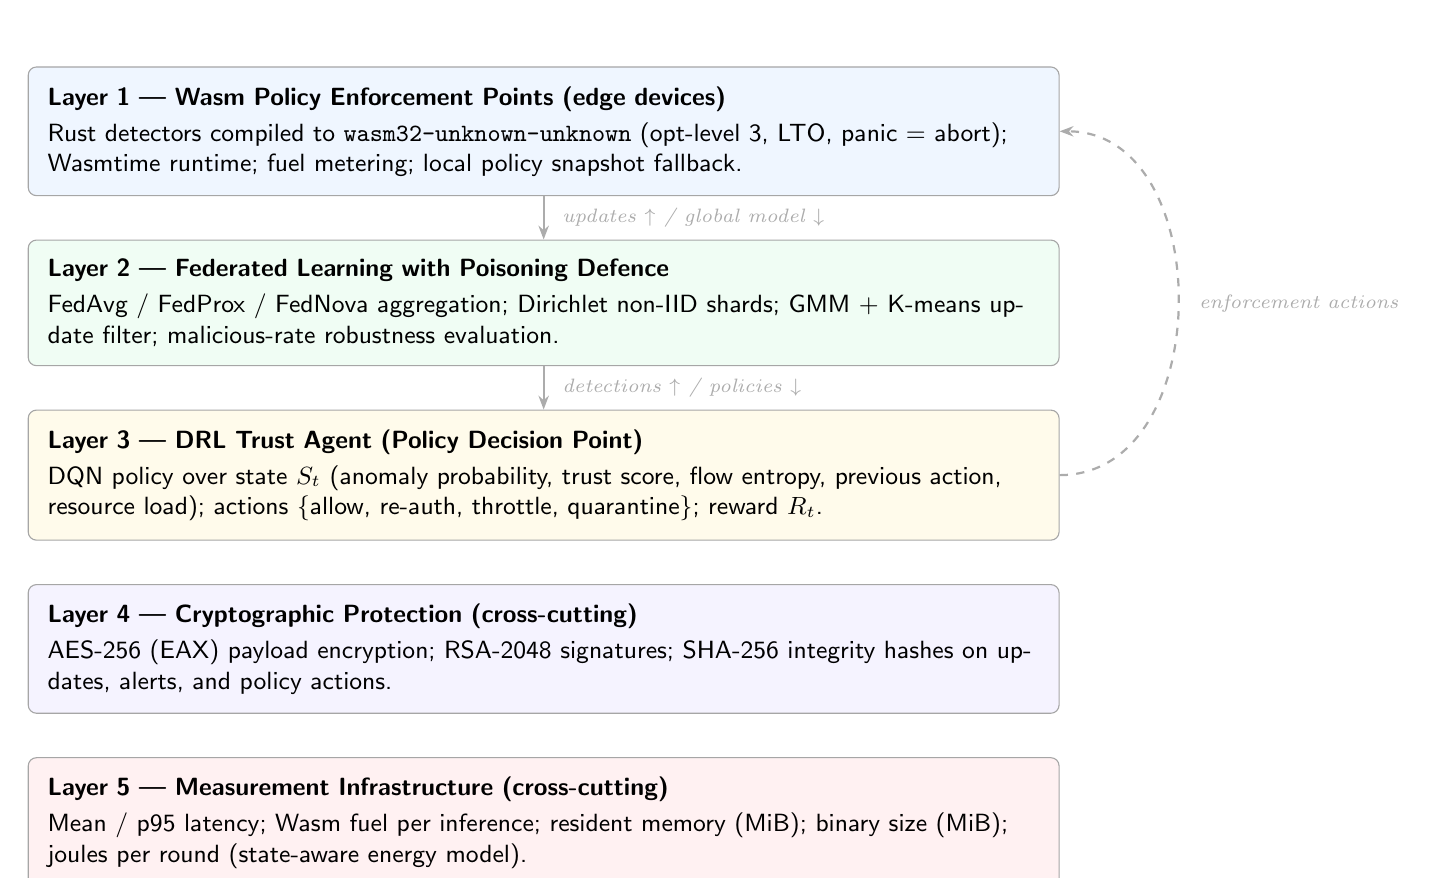
\begin{tikzpicture}[
  layer/.style={draw=gray!70, rounded corners=3pt, text width=12.6cm,
                inner sep=7pt, align=left, font=\small\sffamily},
  arr/.style={-{Stealth[length=5pt]}, thick, gray!65},
  ret/.style={-{Stealth[length=5pt]}, thick, dashed, gray!65}
]
\node[layer, fill=layerblue] (l1)
  {\textbf{Layer 1 --- Wasm Policy Enforcement Points (edge devices)}\\[2pt]
   Rust detectors compiled to \texttt{wasm32-unknown-unknown} (opt-level 3,
   LTO, panic = abort); Wasmtime runtime; fuel metering; local policy
   snapshot fallback.};
\node[layer, fill=layergreen, below=0.55cm of l1] (l2)
  {\textbf{Layer 2 --- Federated Learning with Poisoning Defence}\\[2pt]
   FedAvg / FedProx / FedNova aggregation; Dirichlet non-IID shards;
   GMM + K-means update filter; malicious-rate robustness evaluation.};
\node[layer, fill=layeramber, below=0.55cm of l2] (l3)
  {\textbf{Layer 3 --- DRL Trust Agent (Policy Decision Point)}\\[2pt]
   DQN policy over state $S_t$ (anomaly probability, trust score, flow
   entropy, previous action, resource load); actions \{allow,
   re-auth, throttle, quarantine\}; reward $R_t$.};
\node[layer, fill=layerviolet, below=0.55cm of l3] (l4)
  {\textbf{Layer 4 --- Cryptographic Protection (cross-cutting)}\\[2pt]
   AES-256 (EAX) payload encryption; RSA-2048 signatures; SHA-256
   integrity hashes on updates, alerts, and policy actions.};
\node[layer, fill=layerrose, below=0.55cm of l4] (l5)
  {\textbf{Layer 5 --- Measurement Infrastructure (cross-cutting)}\\[2pt]
   Mean / p95 latency; Wasm fuel per inference; resident memory (MiB);
   binary size (MiB); joules per round (state-aware energy model).};
\draw[arr] (l1) -- (l2) node[midway, right=3pt, font=\scriptsize\itshape]
  {updates $\uparrow$ / global model $\downarrow$};
\draw[arr] (l2) -- (l3) node[midway, right=3pt, font=\scriptsize\itshape]
  {detections $\uparrow$ / policies $\downarrow$};
\draw[ret] (l3.east) .. controls +(2.0,0) and +(2.0,0) .. (l1.east)
  node[midway, right=4pt, font=\scriptsize\itshape, text width=2.6cm]
  {enforcement actions};
\end{tikzpicture}}
\caption{The five-layer FedZT-Edge architecture. Layers 1--3 form the
detection--learning--decision loop; Layers 4 and 5 cut across all
execution paths.}
\label{fig:arch}
\end{figure}

\begin{figure}[htbp]
\centering
\resizebox{0.98\textwidth}{!}{%
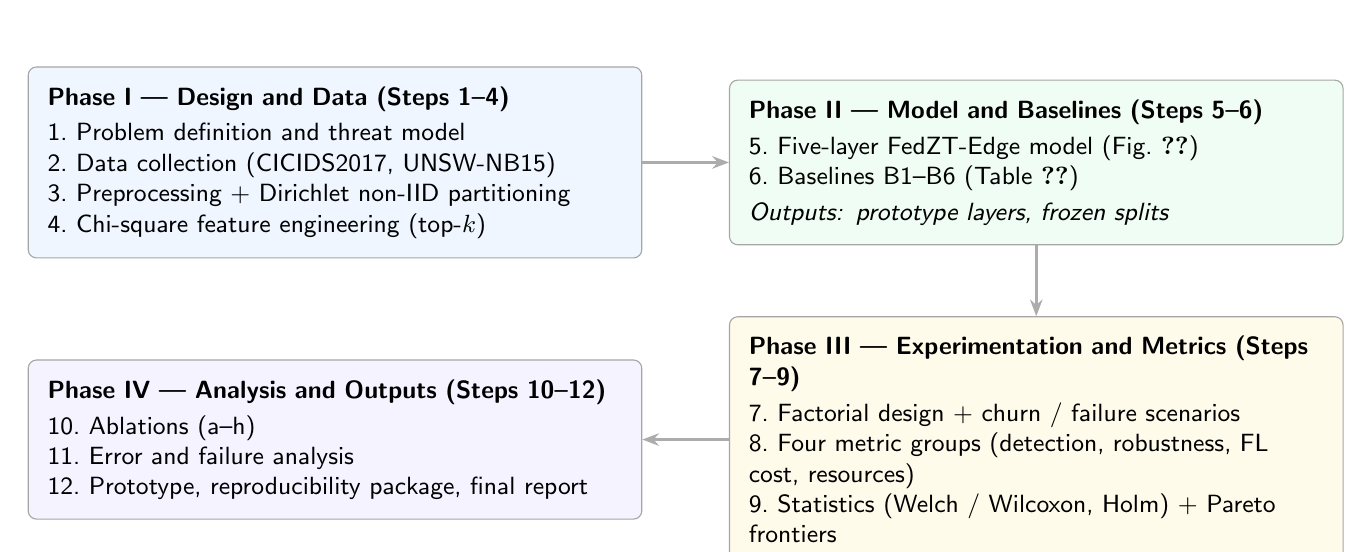
\begin{tikzpicture}[
  phase/.style={draw=gray!70, rounded corners=3pt, text width=7.3cm,
                inner sep=7pt, align=left, font=\small\sffamily},
  arr/.style={-{Stealth[length=6pt]}, very thick, gray!65}
]
\node[phase, fill=layerblue] (p1)
  {\textbf{Phase I --- Design and Data (Steps 1--4)}\\[2pt]
   1.\ Problem definition and threat model\\
   2.\ Data collection (CICIDS2017, UNSW-NB15)\\
   3.\ Preprocessing + Dirichlet non-IID partitioning\\
   4.\ Chi-square feature engineering (top-$k$)};
\node[phase, fill=layergreen, right=1.1cm of p1] (p2)
  {\textbf{Phase II --- Model and Baselines (Steps 5--6)}\\[2pt]
   5.\ Five-layer FedZT-Edge model (Fig.~\ref{fig:arch})\\
   6.\ Baselines B1--B6 (Table~\ref{tab:baselines})\\[2pt]
   \emph{Outputs: prototype layers, frozen splits}};
\node[phase, fill=layeramber, below=0.9cm of p2] (p3)
  {\textbf{Phase III --- Experimentation and Metrics (Steps 7--9)}\\[2pt]
   7.\ Factorial design + churn / failure scenarios\\
   8.\ Four metric groups (detection, robustness, FL cost, resources)\\
   9.\ Statistics (Welch / Wilcoxon, Holm) + Pareto frontiers};
\node[phase, fill=layerviolet, left=1.1cm of p3] (p4)
  {\textbf{Phase IV --- Analysis and Outputs (Steps 10--12)}\\[2pt]
   10.\ Ablations (a--h)\\
   11.\ Error and failure analysis\\
   12.\ Prototype, reproducibility package, final report};
\draw[arr] (p1) -- (p2);
\draw[arr] (p2) -- (p3);
\draw[arr] (p3) -- (p4);
\end{tikzpicture}}
\caption{The twelve-step methodology grouped into four phases. Phase
order follows the numbering of the subsections in
Section~\ref{sec:method}.}
\label{fig:pipeline}
\end{figure}

% ============================================================================
\bigsection{Verification Notes and Threats to Validity}\label{sec:validity}
% ============================================================================

Three verification caveats accompany this report, and each one is
deliberately visible rather than hidden. First, the entries for
Refs.~\cite{rezaei2025,bensaid2025,nandanwar2025} rest on titles,
abstracts, and publisher metadata because no legal open-access full text
exists under the FAST-NUCES access constraints; their table rows are
dagger-flagged in Table~\ref{tab:comparison} and their claims are used
only qualitatively, never as quantitative baselines. Second, the Wasm
survey was reviewed from its arXiv v2 preprint
(Ref.~\cite{zhang2025}); the ACM TOSEM version of record may differ
slightly in coverage counts, and any figure cited from it in the final
thesis should be re-verified against the published version if library
access becomes available. Third, all quantitative cells for the seven
full-text studies were extracted programmatically from the downloaded
PDFs and cross-checked against their abstracts, a process that corrected
several earlier draft inferences --- most notably the detector family of
Ref.~\cite{albogami2025}, which is a federated hybrid deep belief network
rather than a CNN--RNN combination. These controls do not eliminate the
risk of misreading a paywalled source, but they bound it to the three
flagged rows and keep every other claim independently checkable.

% ============================================================================
% REFERENCES
% Entries [1]-[3] are the Phase 1 core papers; entries [4]-[13] are the ten
% new studies reviewed in this phase. Verify the three "% TODO" entries
% against your Phase 1 report before submission.
% ============================================================================
\begin{thebibliography}{13}
\raggedright

% TODO: complete the author list from your Phase 1 copy of the paper.
\bibitem{flexids}
A.~P. Chowdhury et~al.,
``FLEX-IDS: A secure and explainable federated intrusion detection framework
for Edge-of-Things environments under adversarial conditions,''
\emph{Computers and Electrical Engineering}, 2026.
DOI: 10.1016/j.compeleceng.2025.110827.

% TODO: verify exact title wording, volume, and page numbers from your
% Phase 1 copy of the paper.
\bibitem{mahida2026}
A.~Mahida et~al.,
``An intellectual zero trust security framework using deep reinforcement
learning for predictive threat mitigation,''
\emph{IEEE Access}, vol.~14, 2026.

% TODO: verify exact page range from your Phase 1 copy of the paper.
\bibitem{weber2026}
J.~Weber et~al.,
``Lightweight WebAssembly-based intrusion detection for zero trust edge
networks,''
\emph{IEEE Access}, vol.~14, pp.~35337--35355, 2026.
DOI: 10.1109/ACCESS.2026.11411776.

\bibitem{rezaei2025}
H.~Rezaei, R.~Taheri, I.~Jordanov, and M.~Shojafar,
``Federated RNN for intrusion detection system in IoT environment under
adversarial attack,''
\emph{Journal of Network and Systems Management}, vol.~33, no.~4, art.~82,
2025. DOI: 10.1007/s10922-025-09963-8.

\bibitem{bensaid2025}
R.~Bensaid, N.~Labraoui, H.~Saidi, and H.~Bany Salameh,
``Securing fog-assisted IoT smart homes: a federated learning-based
intrusion detection approach,''
\emph{Cluster Computing}, vol.~28, 2025.
DOI: 10.1007/s10586-024-04711-0.

\bibitem{albogami2025}
N.~N. Albogami,
``Intelligent deep federated learning model for enhancing security in
internet of things enabled edge computing environment,''
\emph{Scientific Reports}, vol.~15, art.~4041, 2025.
DOI: 10.1038/s41598-025-88163-5.

\bibitem{karunamurthy2025}
A.~Karunamurthy, K.~Vijayan, P.~R. Kshirsagar, and K.~T. Tan,
``An optimal federated learning-based intrusion detection for IoT
environment,''
\emph{Scientific Reports}, vol.~15, art.~8696, 2025.
DOI: 10.1038/s41598-025-93501-8.

\bibitem{nandanwar2025}
H.~Nandanwar et~al.,
``A hybrid blockchain-based framework for securing intrusion detection
systems in internet of things,''
\emph{Cluster Computing}, vol.~28, art.~472, 2025.
DOI: 10.1007/s10586-025-05135-0.

\bibitem{berguiga2025}
A.~Berguiga, A.~Harchay, and A.~Massaoudi,
``HIDS-IoMT: A deep learning-based intelligent intrusion detection system
for the Internet of Medical Things,''
\emph{IEEE Access}, vol.~13, 2025.
DOI: 10.1109/ACCESS.2025.3543127.

\bibitem{zhang2025}
Y.~Zhang, M.~Liu, H.~Wang, Y.~Ma, G.~Huang, and X.~Liu,
``Research on WebAssembly runtimes: A survey,''
\emph{ACM Transactions on Software Engineering and Methodology}, vol.~34,
2025. DOI: 10.1145/3714465. Preprint: arXiv:2404.12621v2.

\bibitem{djemaa2026}
A.~Djemaa, D.~Djenouri, and P.~Legg,
``Heterogeneity-aware poisoning attacks and mitigation in federated
learning: A comprehensive survey and taxonomy,''
\emph{Electronics}, vol.~15, no.~13, art.~2876, 2026.
DOI: 10.3390/electronics15132876.

\bibitem{hozouri2025}
A.~Hozouri, A.~Mirzaei, and M.~Effatparvar,
``A comprehensive survey on intrusion detection systems with advances in
machine learning, deep learning and emerging cybersecurity challenges,''
\emph{Discover Artificial Intelligence}, vol.~5, art.~314, 2025.
DOI: 10.1007/s44163-025-00578-1.

\bibitem{diana2025}
L.~Diana, P.~Dini, and D.~Paolini,
``Overview on intrusion detection systems for computers networking
security,''
\emph{Computers}, vol.~14, no.~3, art.~87, 2025.
DOI: 10.3390/computers14030087.

\end{thebibliography}

% ----------------------------------------------------------------------------
% PDF metadata is configured in the preamble (see \hypersetup).
% ----------------------------------------------------------------------------

\end{document}
